% !TeX program = xelatex
%! Author = breandan
%! Date = 8/7/26

\documentclass[11pt]{beamer}

\usepackage{amsmath}
\usepackage{pgfplots}
\pgfplotsset{compat=1.18}

\usepackage[normalem]{ulem}
\usepackage{graphicx}
\usepackage[outline]{contour} % Adds synthetic boldness to text

% Set how much thicker you want the line to be
\contourlength{0.25pt}

\makeatletter
\@ifundefined{tenly}{\font\tenly=lasy10}{}
\def\squigglyred{%
  \bgroup
  % We wrap the \char58 in \contour{red}{...} to thicken the stroke
  \markoverwith{\textcolor{red}{\lower5.5\p@\hbox{\scalebox{0.5}[0.85]{\contour{red}{\tenly \char58}}}}}%
  \ULon
}
\makeatother

\newcommand{\err}[1]{%
  \ifmmode
    \text{\squigglyred{$#1$}}%
  \else
    \squigglyred{#1}%
  \fi
}

% Preamble additions
\usepackage{fontspec}
\setmonofont{JetBrainsMono}[
  Path=font/,
  Extension=.ttf,
  UprightFont=*-Regular,
  BoldFont=*-Bold,
  ItalicFont=*-Italic,
  BoldItalicFont=*-BoldItalic
]
\usepackage{amsmath}
\usepackage{array}
\usepackage{listings}

\definecolor{grammarcodekw}{RGB}{74,92,126}
\definecolor{grammarcodecom}{RGB}{105,113,122}
\definecolor{grammarcodestr}{RGB}{118,87,105}
\definecolor{grammarcodetokbg}{RGB}{225,227,230}
\definecolor{grammardivider}{RGB}{190,194,200}

\lstdefinestyle{grammarcpp}{
  language=C++,
  basicstyle=\ttfamily\fontsize{8.0}{10.0}\selectfont,
  keywordstyle=\bfseries\color{grammarcodekw},
  commentstyle=\itshape\color{grammarcodecom},
  stringstyle=\color{grammarcodestr},
  showstringspaces=false,
  keepspaces=true,
  columns=fullflexible
}

% A literal terminal in a grammar production.
\ExplSyntaxOn
\seq_new:N \l__api_gtok_parts_seq
\cs_new_protected:Npn \api_gtok_highlight:n #1
  {
    \seq_set_split:Nnn \l__api_gtok_parts_seq { ~ } {#1}
    \seq_map_indexed_inline:Nn \l__api_gtok_parts_seq
      {
        \int_compare:nNnT {##1} > {1}
          {\hspace{\fontdimen2\font}}
        \tl_if_blank:nF {##2}
          {
            \group_begin:
              \setlength{\fboxsep}{0.2pt}
              \rlap{%
                \kern-0.2pt%
                \smash{\colorbox{grammarcodetokbg}{\vphantom{Ag}\phantom{##2}}}%
              }%
              ##2
            \group_end:
          }
      }
  }
\NewDocumentCommand{\gtok}{m}
  {\mathord{\text{\ttfamily\api_gtok_highlight:n{#1}}}}
\ExplSyntaxOff

% An unhighlighted monospace label used in grammar-name subscripts.
\newcommand{\gsub}[1]{\mathord{\text{\ttfamily #1}}}

% Overlay-aware grammar row. \uncover reserves the row's space from
% slide 1, so neither the code nor the visible mathematics moves.
\newcommand<>{\grow}[1]{%
  \uncover#2{%
    \raisebox{0.15ex}{%
      {\fontsize{8.0}{9.8}\selectfont
        \(\displaystyle #1\)}%
    }%
  }%
}

\title{Compiling Typed APIs\\ into Context-Free Languages	}
\author{Breandan Considine, \textcolor{black!30}{Clemente Pasti, Tim Viera}}
\date{\today}

\begin{document}

% -------------------------------------------------
  \begin{frame}
    \titlepage
  \end{frame}
% -------------------------------------------------

  \begin{frame}{How long are typical source code statements?}
    \begin{figure}
      \centering
      \begin{tikzpicture}
        \begin{axis}[
          width=\textwidth,
          height=0.60\textheight,
          ymin=0,
          ymax=80,
          ytick={0,20,40,60,80},
          ylabel={Mean lexical tokens},
          ylabel style={font=\small},
          symbolic x coords={Java,Kotlin,C,C++,C\#,Rust},
          xtick=data,
          xticklabel style={font=\small},
          yticklabel style={font=\small},
          axis x line*=bottom,
          axis y line*=left,
          axis line style={black!55},
          tick style={black!55},
          ymajorgrids=true,
          grid style={black!10},
          tick align=outside,
          bar width=9mm,
          enlarge x limits=0.10,
        ]

% Bars are means of per-file statement means.
% Error bars are 95% CIs over sampled files.
%
% Java:   mean=16.511928, ci95=9.983352,  n_files=127, n_statements=49923
% Kotlin: mean=24.819900, ci95=6.606195,  n_files=100, n_statements=7197
% C++:    mean=10.530586, ci95=0.526006,  n_files=100, n_statements=60892
% C:      mean=11.317088, ci95=2.872475,  n_files=100, n_statements=78855
% Rust:   mean=36.094937, ci95=25.740138, n_files=100, n_statements=25013
% C#:     mean=12.413997, ci95=1.753571,  n_files=100, n_statements=37004

          \addplot+[
          ybar,
          fill=blue!28!gray,
          draw=blue!45!black,
          line width=0.45pt,
          error bars/.cd,
          y dir=both,
          y explicit,
          error bar style={
            draw=black!75,
            line width=1.1pt,
          },
          error mark=|,
          error mark options={
            draw=black!75,
            line width=1.1pt,
            mark size=4pt,
          },
          ] coordinates {
            (Java,   16.511928) +- (0,9.983352)
            (Kotlin, 24.819900) +- (0,6.606195)
            (C,      11.317088) +- (0,2.872475)
            (C++,    10.530586) +- (0,0.526006)
            (C\#,    12.413997) +- (0,1.753571)
            (Rust,   36.094937) +- (0,25.740138)
          };

% Number of sampled files.
          \node[font=\scriptsize, text=black!65, anchor=north]
          at (axis cs:Java,0) [yshift=-18pt] {$n=127$};
          \node[font=\scriptsize, text=black!65, anchor=north]
          at (axis cs:Kotlin,0) [yshift=-18pt] {$n=100$};
          \node[font=\scriptsize, text=black!65, anchor=north]
          at (axis cs:C++,0) [yshift=-18pt] {$n=100$};
          \node[font=\scriptsize, text=black!65, anchor=north]
          at (axis cs:C,0) [yshift=-18pt] {$n=100$};
          \node[font=\scriptsize, text=black!65, anchor=north]
          at (axis cs:Rust,0) [yshift=-18pt] {$n=100$};
          \node[font=\scriptsize, text=black!65, anchor=north]
          at (axis cs:C\#,0) [yshift=-18pt] {$n=100$};

        \end{axis}
      \end{tikzpicture}

      \caption{Whiskers are 95\% CIs over sampled files. Statements are Tree-sitter statement nodes with comments and whitespace ignored. Sample size is 100 random GitHub files per language $>20$kb.}
    \end{figure}
  \end{frame}

  \begin{frame}{Motivation}
    \begin{itemize}
      \item Construct a $\ell_\Gamma = \mathcal{L}(G_\Gamma)$ consisting of well-typed statements
      \item No well-typed statement $\sigma \notin \ell_\Gamma$ or ill-typed statements $\err{\sigma} \in \ell_\Gamma$
      \item For any $\sigma$ such that $\exists\tau. \sigma\tau \in \ell_\Gamma$, display $\tau$'s in shortlex order
    \end{itemize}
  \end{frame}

  \begin{frame}[t,fragile]{Grammar Modularization}
    \lstset{style=grammarcpp}
    \setlength{\tabcolsep}{0pt}
    \renewcommand{\arraystretch}{0.95}
    \fontsize{8.0}{9.2}\selectfont
    \newcommand{\codecursor}{%
      \makebox[0pt][l]{%
        \smash{\raisebox{-0.18ex}{\rule{0.55pt}{3ex}}}%
      }%
    }
    \hspace*{-0.06\textwidth}%
    \begin{tabular}{@{}
        >{\raggedright\arraybackslash
      \leavevmode\lower1.5ex\hbox\bgroup}
      p{0.55\textwidth}
        <{\egroup}
      @{\hspace{0.012\textwidth}%
      {\color{grammardivider}\vrule width 0.45pt}%
      \hspace{0.012\textwidth}}
        >{\raggedright\arraybackslash}p{0.55\textwidth}
      @{}
    }
      \multicolumn{1}{@{}l}{\scriptsize\bfseries C++ context}
      & {\scriptsize\bfseries Grammar contribution} \\[0.25ex]
      \cline{1-1}\cline{2-2}

      \lstinline!// Filetype: *.cpp!
      & \grow<1->{G_{\gsub{C++}}\:\cup} \\

      \lstinline!#include <string>!
      & \grow<2->{G_{\gsub{<string>}}\:\cup} \\

      \lstinline!#include <vector>!
      & \grow<3->{G_{\gsub{<vector>}}\:\cup} \\

      \lstinline!#include "org/fizz.hpp"!
      & \grow<4->{G_{\gsub{org/fizz.hpp}}\:\cup} \\

      \lstinline!#include "com/buzz.hpp"!
      & \grow<5->{G_{\gsub{com/buzz.hpp}}\:\cup} \\

      \lstinline!using std::string;!
      & \grow<6->{%
        \{\,\mathsf{Type} \to \gtok{string}\,\}\:\cup
      } \\

      \lstinline!// ...!
      & \grow<7->{\cdots} \\

      \lstinline!int fizz() { return 3; }!
      & \grow<8->{%
        \{\,\mathsf{Int}\to\gtok{fizz()},\;
        \mathsf{S}\to\gtok{fizz();}\,\}\:\cup
      } \\

      \lstinline!string buzz(string s) { return s; }!
      & \grow<9->{%
        \{\,\mathsf{Str}\to
        \gtok{buzz( }\mathsf{Str}\gtok{ )},\;
        \mathsf{S}\to
        \gtok{buzz( }\mathsf{Str}\gtok{ );}\,\}\:\cup\hspace{-5cm}
      } \\

      \lstinline!// ...!
      & \grow<10->{\cdots} \\

      \lstinline!int main(int argc, char* args[]) {!
      & \grow<11->{%
        \{\,\mathsf{Int}\to \gtok{argc},
        \,\mathsf{CharPtr}\to
        \gtok{args[ }\mathsf{Int}\gtok{ ]}\,\}\:\cup
      } \\

      \lstinline!  string bang = "...";!
      & \grow<12->{%
        \{\,\mathsf{Str}\to\gtok{bang}\,\} \color{black!30}{\,\:\rightarrow G_\Gamma}
      } \\

      \lstinline!  !\codecursor
      & \grow<13->{L(G_{\Gamma})} \\

      \lstinline!}!
      & \\
    \end{tabular}
  \end{frame}

  \begin{frame}{Monomorphization}
    % TODO
  \end{frame}

  \begin{frame}{Covariance and contravariance}
    % TODO
  \end{frame}

  \begin{frame}{Results: Size of generated CFGs}
    % TODO
  \end{frame}
\end{document}
